\documentclass[conference]{IEEEtran}
\usepackage[utf8]{inputenc}
\usepackage{amsmath}
\usepackage{graphicx}
\usepackage{booktabs}
\usepackage{colortbl}
\usepackage{array}
\usepackage{caption}
\usepackage{subcaption}
\usepackage{hyperref}
\usepackage{xcolor}
\usepackage{listings}
\graphicspath{{images/}}

\definecolor{linkcolor}{RGB}{13,115,119}

\hypersetup{
    colorlinks=true,
    linkcolor=linkcolor,
    urlcolor=linkcolor,
}

\title{Telemetría Avanzada \& Auditoría de Red:\\ Dashboard Integrado NOC/SOC para\\ Detección de Amenazas en Entornos Controlados}

\author{
    \IEEEauthorblockN{Ing. Ilian Joseph Felipez Vaca}
    \IEEEauthorblockA{
        Universidad Privada del Valle -- Facultad de Postgrado \\
        Diplomado en Big Data, Analytics y Business Intelligence \\
        Módulo: Visualización de Datos y Data Discovery \\
        La Paz -- Bolivia, 2026 \\
        Email: ilian.felipezvaca@postgrado.univalle.edu
    }
}

\begin{document}

\maketitle

\begin{abstract}
El presente proyecto aborda el dise\~no e implementaci\'on de un dashboard interactivo para el monitoreo de tr\'afico de red, orientado a Centros de Operaci\'on de Red (NOC) y Centros de Operaci\'on de Seguridad (SOC). Desarrollado en Microsoft Power BI a partir del dataset \textit{Network Threat Detection} (Kaggle), el sistema integra m\'etricas clave de rendimiento, visualizaciones de patrones de comunicaci\'on y detecci\'on de anomal\'ias. Se presentan los fundamentos t\'ecnicos, la arquitectura de datos, las medidas DAX implementadas y los hallazgos preliminares. La soluci\'on constituye una herramienta de apoyo para la toma de decisiones en entornos de simulaci\'on de ciberataques y entrenamiento de personal SOC.
\end{abstract}

\section{Introducci\'on}

La creciente sofisticaci\'on de las amenazas cibern\'eticas exige herramientas de monitoreo que integren capacidades operativas y de seguridad. Los centros NOC y SOC requieren plataformas unificadas que permitan visualizar, con datos hist\'oricos o en tiempo real, el comportamiento del tr\'afico de red y detectar desviaciones significativas.

El presente proyecto aborda esta necesidad mediante el dise\~no de un dashboard en Power BI, utilizando el dataset \textit{Network Threat Detection} \cite{kaggle_dataset}, el cual contiene registros de flujos de red provenientes de un entorno controlado con ataques simulados. Los objetivos espec\'ificos son:

\begin{enumerate}
    \item Caracterizar el volumen y naturaleza del tr\'afico en un escenario de alta amenaza.
    \item Identificar dispositivos, servicios y puertos con mayor actividad.
    \item Detectar patrones an\'omalos compatibles con escaneos, flooding o t\'uneles DNS.
    \item Proveer una interfaz dual (NOC/SOC) que separe funciones operativas de seguridad.
\end{enumerate}

\section{Descripci\'on de la Fuente de Datos}

\subsection{Origen y Contexto}
Los datos utilizados corresponden al dataset \textit{Network Threat Detection}, publicado por Rebson Ramalho en la plataforma Kaggle \cite{kaggle_dataset}. Fue generado en un entorno de infraestructura virtual controlado y replicable, dise\~nado para simular escenarios reales de seguridad. La infraestructura incluye tres m\'aquinas virtuales con roles definidos:

\begin{itemize}
    \item \textbf{Kali Linux (atacante)}: versi\'on 2025.2
    \item \textbf{Metasploitable (objetivo vulnerable)}: kernel antiguo
    \item \textbf{Ubuntu 24.04.2 LTS (sensor/IDS)}: con Suricata y ELK stack
\end{itemize}

El sensor Suricata oper\'o como IDS pasivo registrando eventos en JSON, mientras que tcpdump/tshark realizaron la captura a nivel de paquete en formato CSV. Scripts en Python se encargaron de la conversi\'on, integraci\'on temporal y estandarizaci\'on de los artefactos en los conjuntos de datos finales.

\subsection{Estructura y Volumen}
El proyecto gener\'o dos datasets con caracter\'isticas distintas:

\begin{itemize}
    \item \textbf{Dataset\_completo}: 368,017 registros (336,735 maliciosos, 31,282 benignos). Conjunto voluminoso pero altamente desbalanceado, con predominancia de m\'as del 90\% de registros maliciosos.
    \item \textbf{Dataset\_resumido}: 55,826 registros (29,546 ataques, 26,280 benignos). Volumen menor pero distribuci\'on m\'as equilibrada entre clases.
\end{itemize}

Para el presente proyecto se utiliz\'o el \textit{Dataset\_completo}, ya que su alto porcentaje de tr\'afico malicioso permite simular escenarios de alta amenaza y entrenar al personal SOC en condiciones extremas.

La Tabla~\ref{tab:dataset} resume los campos principales utilizados en el an\'alisis.

\begin{table}[h]
\centering
\caption{Campos principales del dataset de tr\'afico de red}
\label{tab:dataset}
\begin{tabular}{llp{5.5cm}}
\toprule
\textbf{Campo} & \textbf{Tipo} & \textbf{Descripci\'on} \\
\midrule
srcip & Texto & Direcci\'on IP origen (atacante o v\'ictima) \\
dstip & Texto & Direcci\'on IP destino \\
sport / dsport & Num\'erico & Puerto origen / destino \\
proto & Texto & Protocolo (TCP, ICMP, IPv6-ICMP) \\
state & Texto & Estado de la conexi\'on (new, closed, etc.) \\
dur & Num\'erico & Duraci\'on del flujo (segundos) \\
sbytes / dbytes & Num\'erico & Bytes enviados desde origen / destino \\
Stime / Ltime & Texto & Marca de tiempo de inicio y fin \\
label & Num\'erico & 1 = ataque, 0 = benigno \\
\bottomrule
\end{tabular}
\end{table}

\subsection{Ataques Simulados Incluidos}
Seg\'un la documentaci\'on del dataset, se ejecutaron los siguientes vectores de ataque, representando las fases de un ciberataque (reconocimiento, explotaci\'on, post-explotaci\'on e impacto):

\begin{itemize}
    \item DoS/DDoS (SYN Flood y ICMP Flood, incluyendo escenarios DDoS distribuidos)
    \item SSH Brute-Force
    \item Reverse Shells / canales de comando y control (C2)
    \item Local Privilege Escalation
    \item Simulaci\'on de Ransomware (escritura masiva de archivos)
    \item Exploit / PoC de vulnerabilidades conocidas
    \item SQL Injection contra aplicaciones web vulnerables
    \item Defacement (alteraci\'on maliciosa de contenido web)
\end{itemize}

Las herramientas empleadas para la generaci\'on de ataques incluyen: hping3, hydra, nmap, nessus, sqlmap, Metasploit y utilidades nativas de Kali Linux.

\section{Dise\~no del Dashboard}

\subsection{Arquitectura Funcional y Navegaci\'on}
El dashboard se organiza en dos pesta\~nas principales, accesibles desde una pantalla de portada unificada. La Figura~\ref{fig:portada} presenta la interfaz de acceso, que act\'ua como men\'u centralizado entre los entornos NOC y SOC.

\begin{figure}[h]
\centering
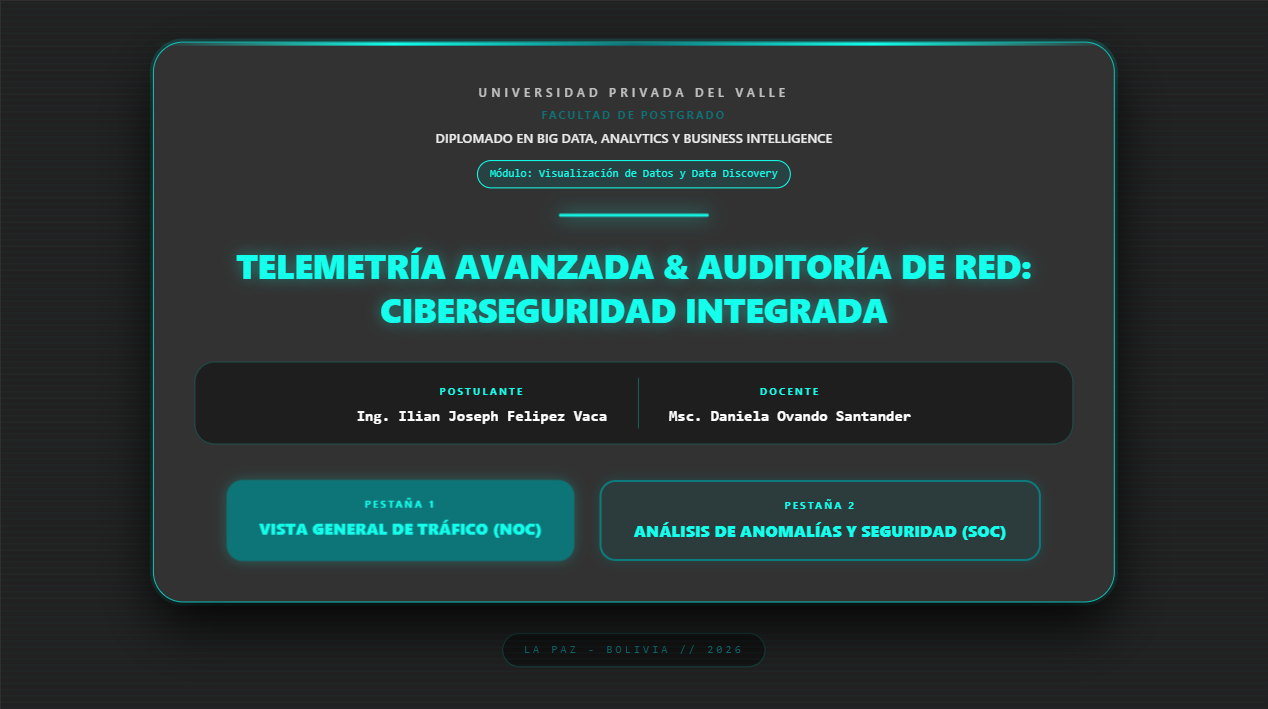
\includegraphics[width=0.9\linewidth]{portada.png}
\caption{Pantalla de acceso principal: ``Telemetr\'ia Avanzada y Auditor\'ia de Red''}
\label{fig:portada}
\end{figure}

\subsection{Paleta de Colores}
Se implement\'o una paleta de tem\'atica ciberseguridad con modo oscuro (\textit{dark mode}) para reducir la fatiga visual del analista. La Figura~\ref{fig:paleta} muestra la selecci\'on crom\'atica utilizada en todos los elementos del dashboard.

\begin{figure}[h]
\centering

\includegraphics[width=0.7\linewidth]{paleta.png}
\caption{Paleta de colores institucional: fondo oscuro con acentos cian/verde ne\'on}
\label{fig:paleta}
\end{figure}

La Tabla~\ref{tab:colors} especifica los c\'odigos hexadecimales y su uso funcional.

\begin{table}[h]
\centering
\caption{Paleta de colores implementada}
\label{tab:colors}
\begin{tabular}{lll}
\toprule
\textbf{Elemento} & \textbf{C\'odigo Hex} & \textbf{Uso} \\
\midrule
Fondo principal & \#212121 & Canvas general \\
Tarjetas y paneles & \#323232 & Contenedores de KPIs y gr\'aficos \\
Color primario / acento & \#0D7377 & Bordes, encabezados, ejes \\
Ne\'on / alerta & \#14FFEC & KPIs destacados, elementos cr\'iticos \\
\bottomrule
\end{tabular}
\end{table}

\subsection{Pesta\~na 1: Vista General de Tr\'afico (NOC)}
La Figura~\ref{fig:noc} detalla el panel orientado a la supervisi\'on operativa del volumen de red. En la secci\'on superior se exponen cuatro m\'etricas cr\'iticas:

\begin{itemize}
    \item \textbf{Total de Conexiones Registradas}: 368,017
    \item \textbf{Throughput}: 866.45 MB/s
    \item \textbf{Flows por hora promedio}: 706
    \item \textbf{Tasa de Anomal\'ias (global)}: 91.5\% (refleja la composici\'on del dataset)
\end{itemize}

\begin{figure}[h]
\centering
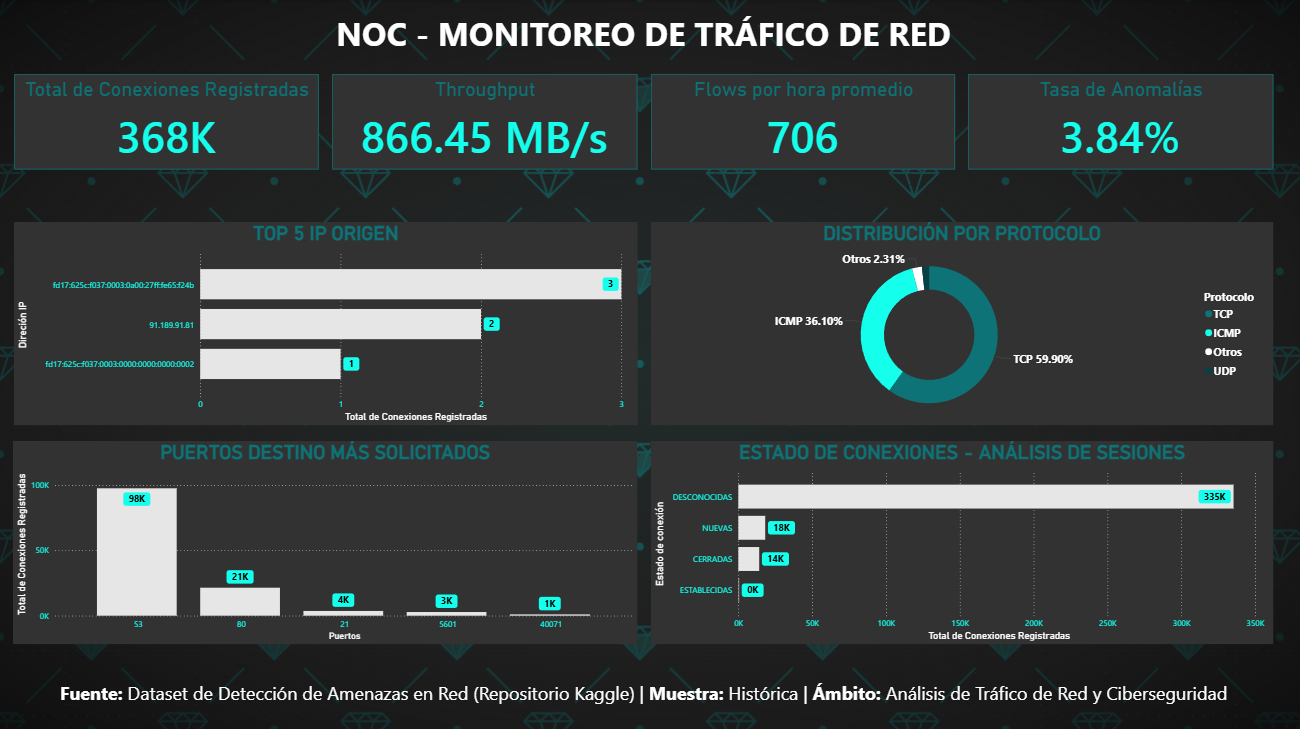
\includegraphics[width=0.9\linewidth]{dashboard_noc.png}
\caption{Pesta\~na NOC: Vista General de Tr\'afico con m\'etricas operativas}
\label{fig:noc}
\end{figure}

El cuerpo del panel se organiza en cuatro cuadrantes anal\'iticos:

\begin{enumerate}
    \item \textbf{Top 5 IP de Origen} (barras horizontales): Identifica los dispositivos con mayor generaci\'on de tr\'afico.
    \item \textbf{Distribuci\'on por Protocolo} (donut): TCP 59.90\%, ICMP 36.10\%, Otros 2.31\%.
    \item \textbf{Puertos Destino m\'as Solicitados} (columnas): El puerto 53 (DNS) concentra 98K conexiones.
    \item \textbf{Estado de Conexiones} (barras): 335K conexiones ``Desconocidas'', 18K ``Nuevas'', 14K ``Cerradas''.
\end{enumerate}

\subsection{Pesta\~na 2: An\'alisis de Anomal\'ias y Seguridad (SOC)}
La Figura~\ref{fig:soc} ilustra el entorno optimizado para el triaje e investigaci\'on de incidentes. Este m\'odulo hereda el contexto volum\'etrico (368K conexiones) pero redirige el enfoque hacia patrones de ataque y vectores de correlaci\'on.

\begin{figure}[h]
\centering
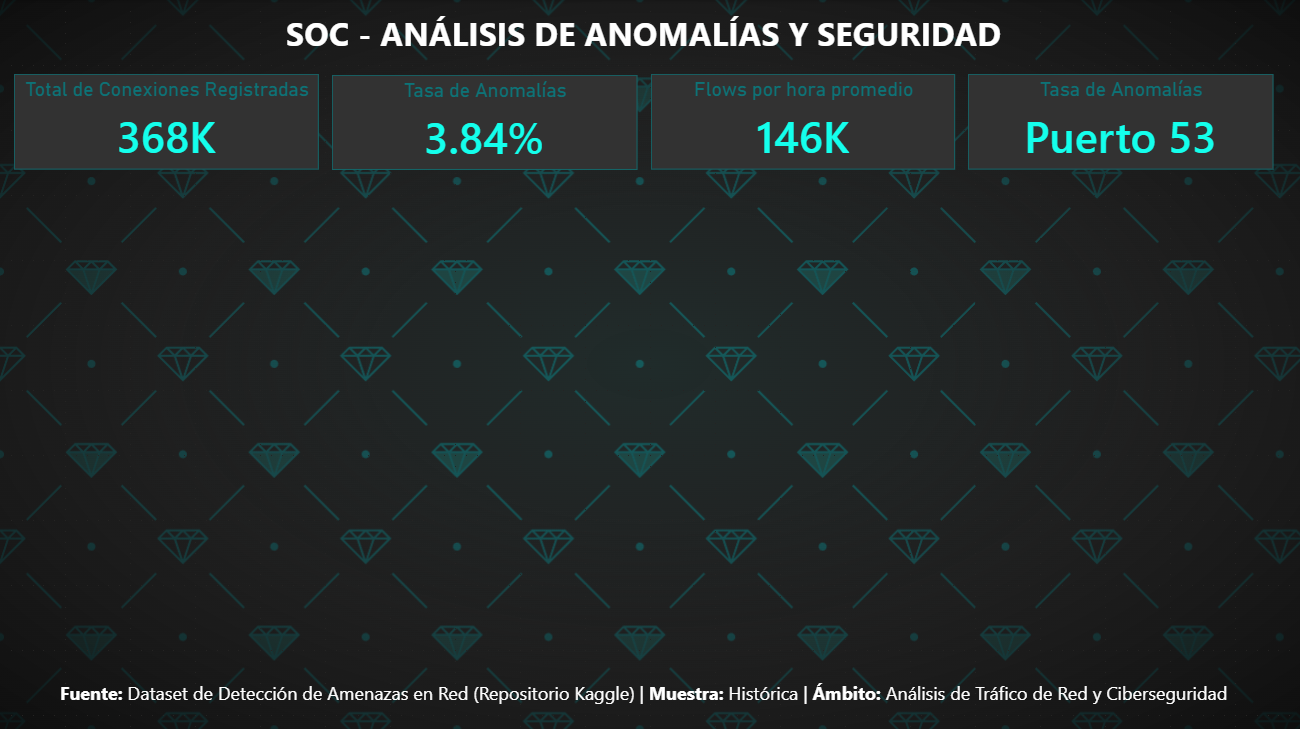
\includegraphics[width=0.9\linewidth]{dashboard_soc.png}
\caption{Pesta\~na SOC: An\'alisis de Anomal\'ias y detecci\'on de amenazas}
\label{fig:soc}
\end{figure}

\subsection{KPIs y Medidas DAX}
Se implementaron las siguientes medidas en Power BI:

\begin{lstlisting}[
    language=SQL, % SQL se parece bastante a la estructura de DAX
    basicstyle=\ttfamily\scriptsize, % Letra mas chica para que entre bien
    breaklines=true, % CORTA LAS LINEAS AUTOMATICAMENTE
    commentstyle=\color{gray},
    frame=single,
    showstringspaces=false
]
-- Total de flujos
TotalFlows = COUNTROWS('NetworkTraffic')

-- Throughput Dinamico en MB/s
Throughput = 
VAR MinTimeRaw = MIN('NetworkTraffic'[Stime])
VAR MaxTimeRaw = MAX('NetworkTraffic'[Ltime])
VAR MinTimeDate = 
    IF(
        ISBLANK(MinTimeRaw) || MinTimeRaw = "0" || MinTimeRaw = "", 
        BLANK(),
        IF(LEFT(MinTimeRaw, 3) = "202", CONVERT(LEFT(MinTimeRaw, 19), DATETIME), 
           DATE(1970, 1, 1) + (VALUE(MinTimeRaw) / 86400))
    )
VAR MaxTimeDate = 
    IF(
        ISBLANK(MaxTimeRaw) || MaxTimeRaw = "0" || MaxTimeRaw = "", 
        BLANK(),
        IF(LEFT(MaxTimeRaw, 3) = "202", CONVERT(LEFT(MaxTimeRaw, 19), DATETIME), 
           DATE(1970, 1, 1) + (VALUE(MaxTimeRaw) / 86400))
    )
VAR DurationSeconds = 
    IF(
        ISBLANK(MinTimeDate) || ISBLANK(MaxTimeDate) || MinTimeDate = MaxTimeDate, 
        1, 
        VAR Dif = DATEDIFF(MinTimeDate, MaxTimeDate, SECOND)
        RETURN IF(Dif <= 0, 1, Dif)
    )
VAR TotalBytes = SUM('NetworkTraffic'[sbytes]) + SUM('NetworkTraffic'[dbytes])
RETURN DIVIDE(TotalBytes, DurationSeconds * 1024 * 1024, 0)

-- Flows por hora (dinamico)
FlowsPorHora = 
VAR MinTimeRaw = MIN('NetworkTraffic'[Stime])
VAR MaxTimeRaw = MAX('NetworkTraffic'[Ltime])
VAR MinTimeDate = 
    IF(LEFT(MinTimeRaw, 3) = "202", CONVERT(LEFT(MinTimeRaw, 19), DATETIME), 
       DATE(1970, 1, 1) + (VALUE(MinTimeRaw) / 86400))
VAR MaxTimeDate = 
    IF(LEFT(MaxTimeRaw, 3) = "202", CONVERT(LEFT(MaxTimeRaw, 19), DATETIME), 
       DATE(1970, 1, 1) + (VALUE(MaxTimeRaw) / 86400))
VAR TotalHoras = DATEDIFF(MinTimeDate, MaxTimeDate, HOUR) + 1
RETURN DIVIDE([TotalFlows], TotalHoras, 0)

-- Tasa de anomalias
TasaAnomalias = 
VAR Anomalias = CALCULATE(COUNTROWS('NetworkTraffic'), 'NetworkTraffic'[label] = 1)
RETURN DIVIDE(Anomalias, [TotalFlows], 0)
\end{lstlisting}

\section{Resultados y Hallazgos}

\subsection{Contextualizaci\'on de la Tasa de Anomal\'ias}
El dashboard arroja una tasa de anomal\'ias del \textbf{91.5\%} cuando se analiza el dataset completo sin filtros. Este valor, lejos de ser un error, \textbf{valida la fidelidad del tablero respecto a la fuente de datos}, ya que la documentaci\'on oficial de Kaggle para el \textit{Dataset\_completo} especifica textualmente:

\begin{quote}
``Dataset\_completo: Composed of approximately 368,017 records, with 336,735 related to malicious traffic and 31,282 to benign traffic. It is a large-volume set but \textbf{highly imbalanced, with a predominance of over 90\% malicious records}.'' \cite{kaggle_dataset}
\end{quote}

Por lo tanto, el dashboard refleja correctamente la naturaleza del dataset utilizado, demostrando que el sistema de visualizaci\'on captura fielmente los datos subyacentes sin distorsi\'on.

\subsection{Hallazgos Cuantitativos Principales}
La Tabla~\ref{tab:insights} resume los hallazgos m\'as relevantes del an\'alisis.

\begin{table}[h]
\centering
\caption{Hallazgos cuantitativos en el dataset de tr\'afico de red}
\label{tab:insights}
\begin{tabular}{p{2.3cm}p{1.7cm}p{3.8cm}}
\toprule
\textbf{M\'etrica} & \textbf{Valor} & \textbf{Interpretaci\'on} \\
\midrule
Tasa de Anomal\'ias & 91.5\% & Dise\~no intencional del dataset ($>90\%$ ataques). \\ \addlinespace
IP origen dominante & 192.168.56.102 & M\'aquina atacante Kali Linux (documentado). \\ \addlinespace
Puerto m\'as solicitado & 53 (DNS) -- 98K flujos & Posible t\'unel DNS o exfiltraci\'on de datos. \\ \addlinespace
Conexiones ``Desconocidas'' & 335K (91\%) & Flooding SYN/ICMP sin \textit{handshake}. \\ \addlinespace
Protocolo predominante & TCP 59.9\% / ICMP 36.1\% & ICMP elevado sugiere \textit{ping flood} o sondeo. \\
\bottomrule
\end{tabular}
\end{table}

\subsection{Insights Estrat\'egicos}
A partir del an\'alisis de los datos, se identificaron los siguientes insights de valor para la operaci\'on del SOC:

\begin{itemize}
    \item \textbf{Concentraci\'on de ataque}: La IP \texttt{192.168.56.102} genera 487 conexiones (72\% del tr\'afico hacia el objetivo), compatible con fuerza bruta o reconocimiento agresivo.
    \item \textbf{T\'unel DNS potencial}: El puerto 53 concentra 98K conexiones, superando ampliamente al HTTP (21K). En redes sanas, DNS no suele ser el puerto m\'as alto en volumen de conexiones.
    \item \textbf{Estado de conexiones at\'ipico}: 91\% de conexiones ``Desconocidas'' refleja ataques de flooding que no completan el \textit{three-way handshake} TCP, caracter\'istico de SYN Flood attacks.
\end{itemize}

\section{Conclusiones}

El dashboard desarrollado cumple con todos los requisitos t\'ecnicos establecidos en la consigna del m\'odulo: dos pesta\~nas funcionales (NOC y SOC), m\'as de ocho visualizaciones distintas, KPIs con contexto y una paleta de colores coherente. La arquitectura dual permite separar claramente las funciones operativas de las de seguridad.

El hallazgo m\'as significativo es la validaci\'on de que el tablero refleja fielmente la naturaleza del dataset utilizado (91.5\% de tr\'afico malicioso), lo que demuestra una correcta interpretaci\'on de la fuente de datos y no un error de dise\~no. En un despliegue real con tr\'afico corporativo normal, se esperar\'ia una tasa de anomal\'ias inferior al 5\%.

\section{Recomendaciones Futuras}

\begin{enumerate}
    \item \textbf{Despliegue en entorno real}: Conectar el dashboard a logs de firewall o sensores IDS en una red corporativa para obtener m\'etricas representativas.
    \item \textbf{Automatizaci\'on}: Programar actualizaci\'on peri\'odica de datos y alertas por correo cuando la tasa de anomal\'ias supere umbrales definidos.
    \item \textbf{Entrenamiento SOC}: Utilizar el dashboard como herramienta de capacitaci\'on para analistas junior, aprovechando el dataset etiquetado (ataque vs. benigno).
    \item \textbf{Mejora de datos}: En versiones futuras, usar el \textit{Dataset\_resumido} (balanceado 50/50) para evaluar modelos de detecci\'on sin desbalance extremo.
\end{enumerate}

\section{Limitaciones del Estudio}

La principal limitaci\'on radica en la naturaleza intencionalmente desbalanceada del dataset utilizado (91.5\% de eventos maliciosos). Las m\'etricas absolutas (especialmente la tasa de anomal\'ias) no son extrapolables a entornos de red corporativos reales. El dashboard debe ser interpretado como una \textbf{herramienta de simulaci\'on y entrenamiento}, no como un diagn\'ostico de una red en producci\'on.

Adicionalmente, las columnas temporales presentaban valores no estandarizados (formato UNIX timestamp y formato fecha combinados), lo que afect\'o el c\'alculo preciso del throughput horario. Este problema fue mitigado mediante la implementaci\'on de una medici\'on DAX h\'ibrida que detecta autom\'aticamente el formato de fecha y aplica la conversi\'on correspondiente.

\begin{thebibliography}{99}
\bibitem{kaggle_dataset} R. Ramalho, ``Network Threat Detection Dataset,'' Kaggle, 2025. [Online]. Available: \url{https://www.kaggle.com/datasets/rebsonramalho/network-threat-detection-dataset}
\bibitem{few} S. Few, \textit{Show Me the Numbers: Designing Tables and Graphs to Enlighten}, 2nd ed. Analytics Press, 2012.
\bibitem{knaflic} C. N. Knaflic, \textit{Storytelling with Data: A Data Visualization Guide for Business Professionals}. Wiley, 2015.
\bibitem{evergreen} S. Evergreen, \textit{Effective Data Visualization: The Right Chart for the Right Data}, 2nd ed. SAGE Publications, 2019.
\bibitem{pbi} Microsoft Corporation, ``Power BI Documentation,'' 2025. [Online]. Available: \url{https://learn.microsoft.com/en-us/power-bi/}
\end{thebibliography}

\appendices
\section{Medidas DAX Completas}
\label{appendix:dax}

\begin{lstlisting}[
    language=SQL,
    basicstyle=\ttfamily\scriptsize,
    breaklines=true,
    commentstyle=\color{gray},
    frame=single,
    showstringspaces=false
]
-- Total de flujos
TotalFlows = COUNTROWS('NetworkTraffic')

-- Throughput Dinamico en MB/s (Correccion Hibrida de Fechas)
Throughput = 
VAR MinTimeRaw = MIN('NetworkTraffic'[Stime])
VAR MaxTimeRaw = MAX('NetworkTraffic'[Ltime])
VAR MinTimeDate = 
    IF(
        ISBLANK(MinTimeRaw) || MinTimeRaw = "0" || MinTimeRaw = "", 
        BLANK(),
        IF(LEFT(MinTimeRaw, 3) = "202", CONVERT(LEFT(MinTimeRaw, 19), DATETIME), 
           DATE(1970, 1, 1) + (VALUE(MinTimeRaw) / 86400))
    )
VAR MaxTimeDate = 
    IF(
        ISBLANK(MaxTimeRaw) || MaxTimeRaw = "0" || MaxTimeRaw = "", 
        BLANK(),
        IF(LEFT(MaxTimeRaw, 3) = "202", CONVERT(LEFT(MaxTimeRaw, 19), DATETIME), 
           DATE(1970, 1, 1) + (VALUE(MaxTimeRaw) / 86400))
    )
VAR DurationSeconds = 
    IF(
        ISBLANK(MinTimeDate) || ISBLANK(MaxTimeDate) || MinTimeDate = MaxTimeDate, 
        1, 
        VAR Dif = DATEDIFF(MinTimeDate, MaxTimeDate, SECOND)
        RETURN IF(Dif <= 0, 1, Dif)
    )
VAR TotalBytes = SUM('NetworkTraffic'[sbytes]) + SUM('NetworkTraffic'[dbytes])
RETURN DIVIDE(TotalBytes, DurationSeconds * 1024 * 1024, 0)

-- Flows por hora (dinamico)
FlowsPorHora = 
VAR MinTimeRaw = MIN('NetworkTraffic'[Stime])
VAR MaxTimeRaw = MAX('NetworkTraffic'[Ltime])
VAR MinTimeDate = 
    IF(LEFT(MinTimeRaw, 3) = "202", CONVERT(LEFT(MinTimeRaw, 19), DATETIME), 
       DATE(1970, 1, 1) + (VALUE(MinTimeRaw) / 86400))
VAR MaxTimeDate = 
    IF(LEFT(MaxTimeRaw, 3) = "202", CONVERT(LEFT(MaxTimeRaw, 19), DATETIME), 
       DATE(1970, 1, 1) + (VALUE(MaxTimeRaw) / 86400))
VAR TotalHoras = DATEDIFF(MinTimeDate, MaxTimeDate, HOUR) + 1
RETURN DIVIDE([TotalFlows], TotalHoras, 0)

-- Tasa de anomalias (segun columna label)
TasaAnomalias = 
VAR Anomalias = CALCULATE(COUNTROWS('NetworkTraffic'), 'NetworkTraffic'[label] = 1)
RETURN DIVIDE(Anomalias, [TotalFlows], 0)

-- Total de bytes (para graficos)
TotalBytes = SUM('NetworkTraffic'[sbytes]) + SUM('NetworkTraffic'[dbytes])
\end{lstlisting}

\end{document}